\chapter{基于抽象和学习的分布式统计模型检测方法}
\label{ch4}
通过对上一个章节得到的模型进行协同仿真,我们可以得到模型的仿真迹。将仿真迹和需要验证的属性输入到统计模型检测器中,即可以对整个系统的行为进行定量的评估分析。但是,基于统计模型检测的大型系统验证分析将产生大量的仿真迹,并且每一条迹的产生都十分的耗费时间。因此,使用统计模型检测算法对大型系统进行验证效率将十分低下。为了解决这一问题,在这一章我们提出了一种基于抽象和学习的分布式统计模型检测方法来提高统计模型检测的效率。本章的第一小节提出了本方法的技术路线及分布式架构设计;第二小节应用分布式架构对一种经典的统计模型检测算法-贝叶斯区间估计算法\cite{zuliani2013bayesian}进行了分布式实现;第三小节首先介绍了基于抽象和学习的统计模型检测算法,然后给出了该算法的分布式实现和优化;最后一个小节给出了基于抽象和学习的分布式统计模型检测算法的算法分析。此外,该算法的效率及准确性对比将在后面的实验章节给出。
\section{技术路线及分布式架构设计}
在本小节,我们首先给出本方法的技术路线及使用到的分布式架构。本方法针对两个方面对统计模型检测算法进行改进,并使用了主从式的分布式架构来对算法进行分布式设计。
\subsection{技术路线}
\label{sec:roadmap}
对统计模型检测算法的效率有直接影响的因素主要有两个:(1)验证过程中产生的仿真迹的数量;(2)产生单条仿真迹需要的时间。在本章,我们针对这两个因素对统计模型检测的效率进行改进。 图\ref{tech-map}是本章的技术路线图,统计模型检测器主要包含三个组件: \emph{仿真器、 统计模型检测算法和模型检测器}。 \emph{仿真器}产生仿真迹并输入到\emph{模型检测器}之中,\emph{模型检测器}跟根据验证属性来检测该仿真迹是否满足该验证属性,并返回检测结果(1表示满足,0表示不满足)。 \emph{统计模型检测(SMC)算法}收集来自\emph{模型检测器}的检测结果并进行统计分析,并返回验证的最终结果。为了减少验证过程中产生的仿真迹的数量,我们在之前的工作中提出了使用抽象和学习的方法对统计模型检测算法进行改进\cite{jiangkaiqiang2016}并提出了基于抽象和学习的统计模型检测算法,经过多次实验分析,我们发现该方法可以有效减少验证过程中产生的仿真迹。根据论文\cite{younes2005ymer},我们发现统计模型检测算法是可以使用基于主从架构的分布式技术进行改进的,即可以用多个仿真器产生仿真迹并用一个统计模型检测器进行统计分析。因此,我们可以使用分布式技术来减少产生单条仿真迹需要的时间,并且我们进一步基于分布式技术设计了分布式的贝叶斯区间估计算法(BIE)。 在本文中,我们结合了分布式技术及抽象和学习技术提出了基于抽象和学习的分布式统计模型检测算法,该算法同时有效减少了验证过程中产生的仿真迹的数量和产生单条仿真迹需要的时间。
\begin{figure}[htbp]
	{
	\centering	
	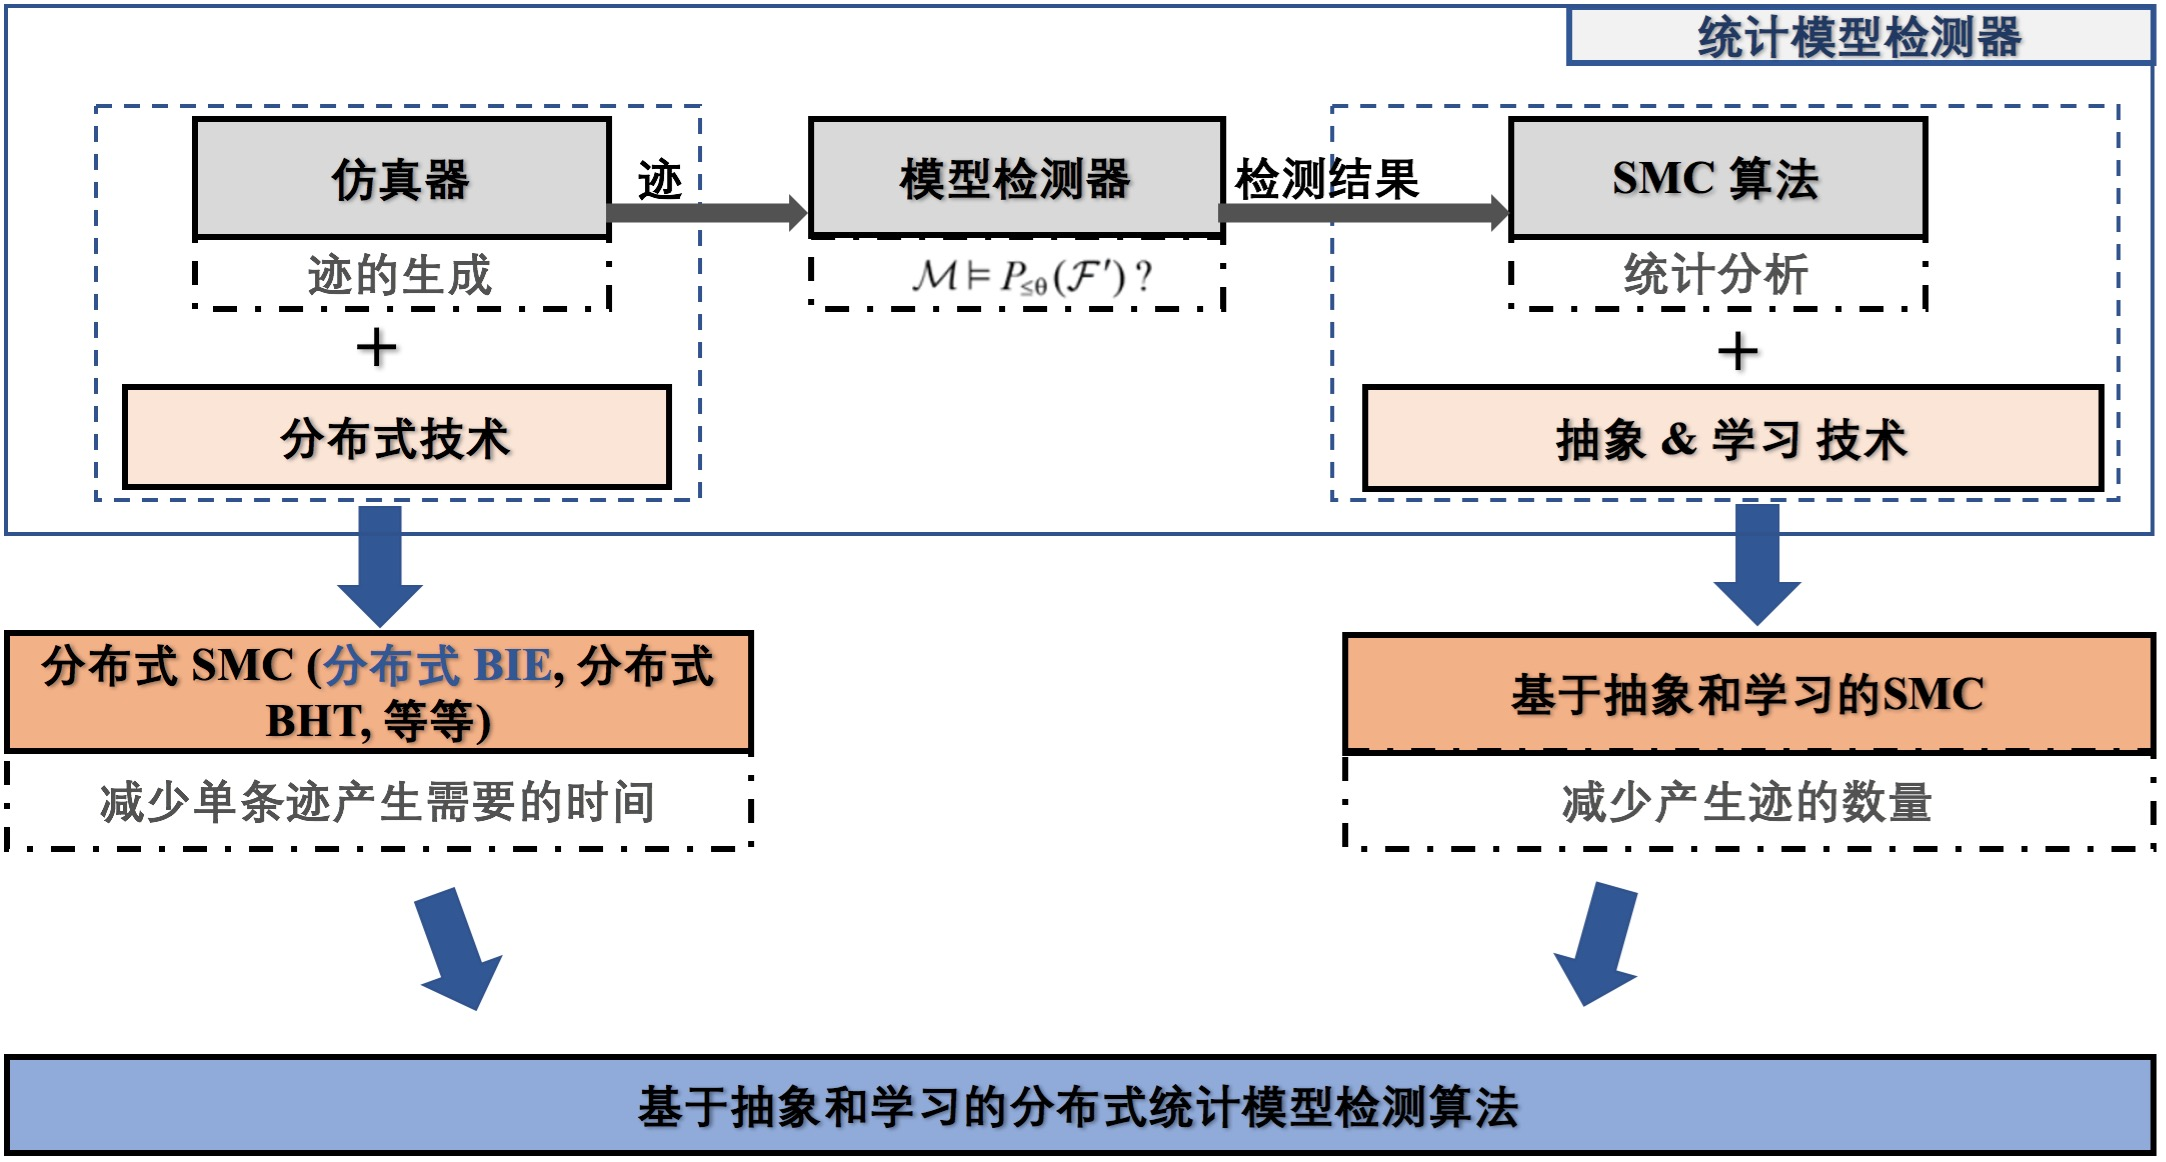
\includegraphics[width=5.0in,height=2.5in]{fig/4/paper-framework.jpg}
\caption{基于抽象和学习的分布式统计模型检测方法技术路线}\label{tech-map}	
	}	
\end{figure}
\subsection{分布式架构设计}
在本小节,我们给出了统计模型检测算法的分布式架构设计如图\ref{fra}所示:多个从属节点进行模型的仿真并产生仿真迹,然后对该仿真迹进行验证并将检测结果(observation)存储到缓冲器(Buffer)中,主节点从缓冲器中收集检测结果并进行统计分析。在对统计模型检测算法进行分布式改进时,有一个关键点就是要避免引入偏差。为了解决这个问题,我们使用了论文 \cite{Bulychev2012Checking}提出的使用缓冲器和批量处理器来避免偏差的方法。

\begin{figure}[htbp]
\centering{
		\subfigure[分布式架构]{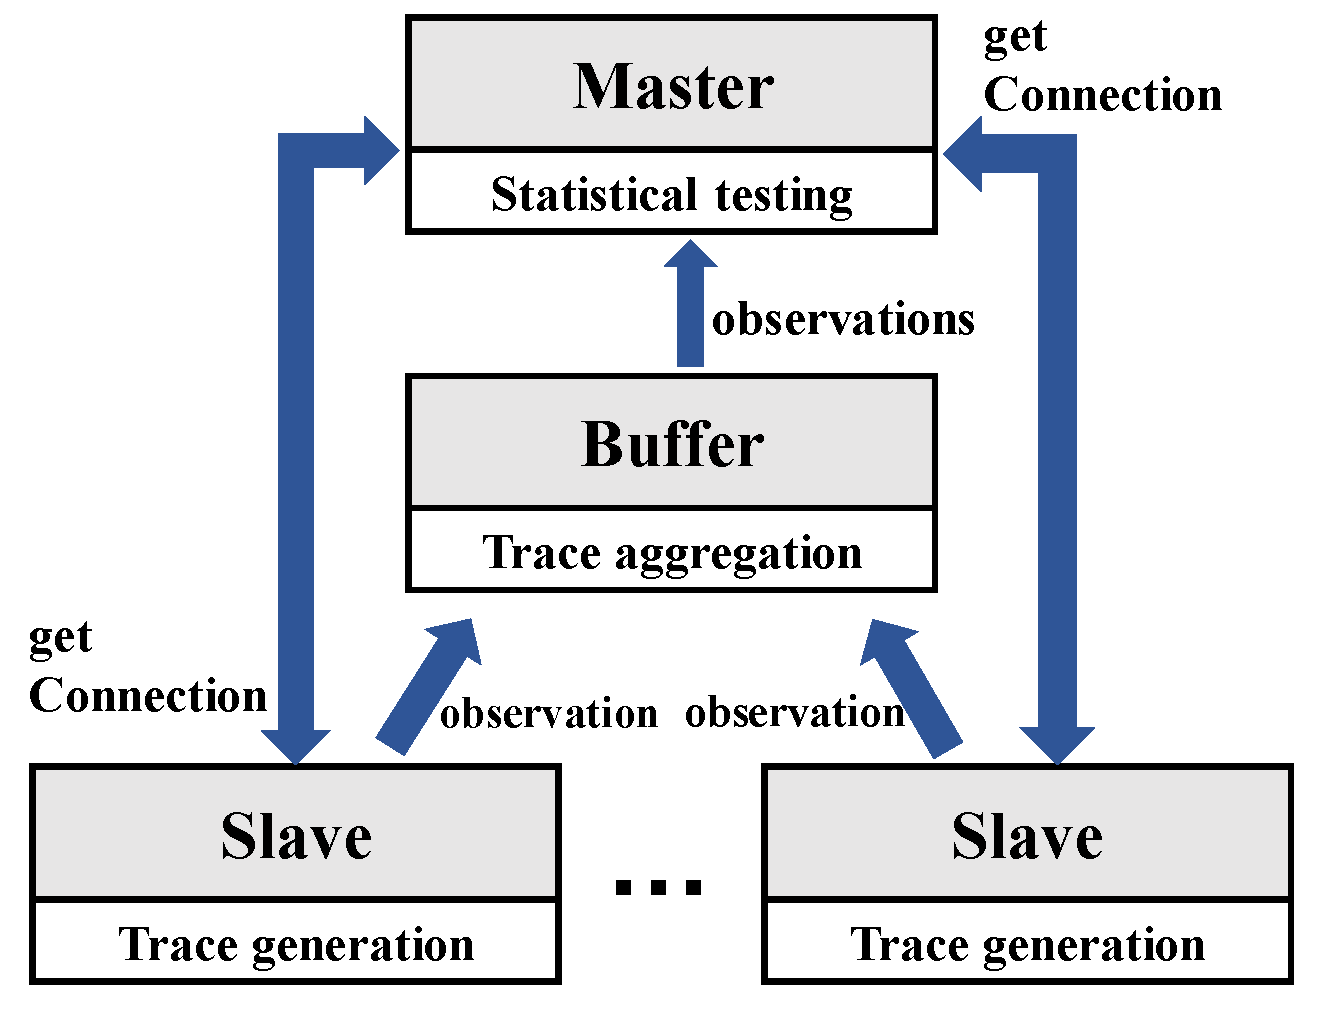
\includegraphics[width=2.5in,height=2.0in]{fig/4/slave-master-ach.png}
			\label{fra}}
		\hfil
		\subfigure[通信协议]{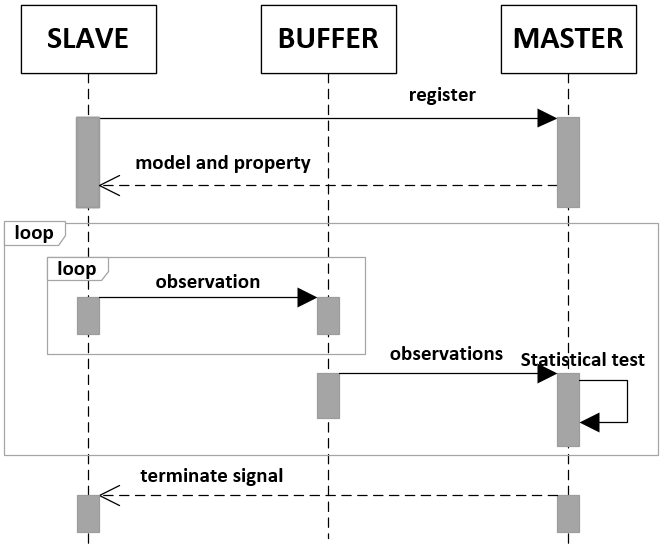
\includegraphics[width=2.5in,height=2.0in]{fig/4/slave-master-seq.png}
			\label{dsmc}}
	\caption{分布式统计模型检测的架构设计}
	\label{fra_dsmc}
	}
\end{figure}
图\ref{dsmc}是分布式统计模型检测的通信时序图: (1)多个从属节点跟主节点建立连接,主节点将模型和验证属性发送给从属节点。(2)从属节点将检测结果发送到缓冲器中,缓冲器中存储的检测结果最终将发送给主节点。 (3)主节点进行统计分析,直到统计分析过程结束,主节点发送终止信号给从属节点,从属节点结束仿真。该分布式统计模型检测算法的分布式框架具有通用性,基于本框架,我们在下个小节设计了分布式的贝叶斯区间估计算法,实际上我们可以将该框架应用到任意一个经典的统计模型检测算法而不只局限于贝叶斯区间估计算法。
\section{分布式的贝叶斯区间估计算法设计}
\label{sec:dbie}
在本小节,我们首先介绍了统计模型检测中一个经典的算法-贝叶斯区间估计算法。之后我们将上一小节提出的分布式框架应用到本算法中,并得到了分布式的贝叶斯区间估计算法。该分布式算法使得贝叶斯区间估计算法产生单条仿真迹的时间有效减少,从而提高了贝叶斯区间估计算法的效率。
\subsection{贝叶斯区间估计算法介绍}
贝叶斯区间估计算法可以用来高效的评估随机模型$M$满足验证属性$\phi$(即,$p=Prob(M\models\phi)$)的概率区间。贝叶斯区间估计算法 (算法 \ref{alg:bie}) 调用仿真器不断的产生仿真迹,然后验证它是否满足验证属性$\phi$并返回检测结果,最后调用统计检测算法(算法 \ref{alg:sta}) 来计算估计概率$p'$,概率区间范围 ($t_0$, $t_1$) 和后置概率$\gamma$。直到满足条件$\gamma >= c$,算法终止并返回$t_0$、$t_1$ 和$p'$的值,否则继续循环产生仿真迹并进行计算。

% Algorithm
\begin{algorithm}
%\SetAlgoNoLine
\begin{algorithmic}[1]
\REQUIRE 验证属性$\phi$、半区间大小$\delta \in (0, 1/2)$、区间覆盖系数$c \in (1/2, 1)$、前置beta分布的参数$\alpha$和$\beta$
\ENSURE 概率区间($t_0$, $t_1$)、估计概率$p'$
\STATE $x$ = 0; $n$ = 0
\LOOP
        \STATE $\sigma$ = draw a simulation of the model
        \IF{$\sigma\models\phi$}
        \STATE $x$ = $x$ + 1
        \ENDIF
        \STATE $n$ = $n$ + 1
        \STATE $t_0$,$t_1$,$p'$,$\gamma$ = \textbf{CallAlgorithm\ref{alg:sta}($\delta$, $\alpha$,$\beta$,$x$, $n$)}
        \IF{$\gamma >= c$}
        \RETURN $t_0$,$t_1$,$p'$,$\gamma$
        \ENDIF
\ENDLOOP
\end{algorithmic}
\caption{贝叶斯区间估计算法}
\label{alg:bie}
\end{algorithm}


% Algorithm
\begin{algorithm}[t]
%\SetAlgoNoLine
\begin{algorithmic}[1]
\REQUIRE 半区间大小$\delta \in (0, 1/2)$、前置beta分布的参数$\alpha$和$\beta$、满足验证属性迹的数量$x$、产生迹的总数量$n$
\ENSURE 概率区间($t_0$, $t_1$)、后置概率$\gamma$、估计概率$p'$
\STATE $p'$ = (x+$\alpha$)/(n+$\alpha$+$\beta$)
\STATE ($t_0$, $t_1$) = ($p^,$-$\delta$,$p^,$+$\delta$)
        \IF{$t_1 > 1$}
        \STATE ($t_0$, $t_1$) = (1-2$\delta$,1)
        \ELSIF{$t_0 > 0$}
        \STATE ($t_0$, $t_1$) = (0,2$\delta$)
        \ENDIF
        \STATE $\gamma=\int_{t_0}^{t_1} {f(u|x_1,...,x_n)du}$
\end{algorithmic}
\caption{统计检测算法}
\label{alg:sta}
\end{algorithm}
\subsection{分布式贝叶斯区间估计算法}
\begin{algorithm}[t]
%\SetAlgoNoLine
\begin{algorithmic}[1]
\REQUIRE 验证属性$\phi$、模型$M$、半区间大小$\delta \in (0, 1/2)$、区间覆盖系数$c \in (1/2, 1)$、前置beta分布的参数$\alpha$和$\beta$、缓冲区大小$K$、批处理区大小$B$、从属节点数量$N$
\ENSURE 概率区间($t_0$, $t_1$)、估计概率$p'$
\STATE $x$ = 0; $n$ = 0
\STATE batch[0...N-1][0...K-1], buffer[0...K-1], slave[0...N-1]
\LOOP 
\STATE getConnection(slave[i])
\STATE sendModelandProperty($M$,$\phi$,slave[i])
\IF{i>N-2}
\RETURN
\ENDIF
\ENDLOOP
\LOOP
        \STATE node = random(0,$N$-1)
        \IF{$buffer[node] < K$}
         \STATE batch[node][buffer[node]] = \textbf{CallAlgorithm\ref{alg:dbeas}(node)}
         \STATE buffer[node]++
         \ENDIF
         \IF{$forall(i < N) buffer[i] > 0$}
         \LOOP
             \STATE x += batch[i][0]
              \STATE n += B
             \STATE buffer[i]--
             \STATE batch[i][buffer[i]] = 0
         \IF{$i > N-1$}
         \RETURN
         \ENDIF
         \ENDLOOP
         \ENDIF
         \STATE $t_0$,$t_1$,$p'$,$\gamma$ = \textbf{CallAlgorithm\ref{alg:sta}($\delta$, $\alpha$,$\beta$ $x$, $n$)}
         \IF{$\gamma >= c$}
         \RETURN $t_0$,$t_1$,$p'$
         \ENDIF
\ENDLOOP
\end{algorithmic}
\caption{分布式贝叶斯区间估计算法的主算法}
\label{alg:dbeam}
\end{algorithm}
% Algorithm
\begin{algorithm}[t]
\begin{algorithmic}[1]
%\SetAlgoNoLine
\REQUIRE 验证属性$\phi$、模型$M$、批处理区大小$B$
\ENSURE 满足验证属性迹的数量$sats$
\STATE $sats$ = 0, $runs$ = 0
\LOOP
        \STATE $\sigma$ := getSimulationTrace($M$)
        \IF{$\sigma \models \phi$}
        \STATE $sats$ ++
        \ENDIF
        \STATE $runs$ ++ 
        \IF{$runs$ == B}
        \RETURN $sats$
        \ENDIF
\ENDLOOP
\end{algorithmic}
\caption{分布式贝叶斯区间估计算法的从算法}
\label{alg:dbeas}
\end{algorithm}
基于贝叶斯区间算法及我们提出的分布式框架,我们设计了分布式的贝叶斯区间估计算法。 算法\ref{alg:dbeas}是分布式贝叶斯区间估计算法的从算法。$B$是批处理分区的大小,用来收集从属节点的仿真结果并存储起来,因此一个从属节点对应的一个批处理分区里面有多个仿真结果。 该算法不断的调用仿真器产生仿真迹并验证该迹是否满足验证属性$\phi$。 直到满足条件$runs == B$,该算法终止并返回满足属性的样本数量$sats$,否则继续循环调用仿真器并验证。

算法\ref{alg:dbeam}是分布式贝叶斯区间估计算法的主算法。 \emph{$K$}是缓冲器的大小,用来缓冲来自某个仿真器的批处理分区,如果有某个仿真器产生迹的速度较快,可以将其批处理分区缓冲到该仿真器对应的缓冲区内,且存储的数量不能超过\emph{$K$}。主算法的主要步骤如下:(1)从属节点与主节点建立连接,主节点将模型和验证属性发送给从属节点。 (2)主算法随机选择一个从算法,如果该从算法的从属节点对应的缓冲区的大小没有超过\emph{$K$},则调用该从算法。(3)如果缓冲器中所有的缓冲区都不为空,则获取缓冲区的验证结果并更新\emph{$n$}和\emph{$x$}的值。 (4)调用算法\ref{alg:sta}来计算估计概率$p'$、概率区间($t_0$, $t_1$) 和后置概率$\gamma$。直到满足条件$\gamma >= c$,算法终止并返回$t_0$、$t_1$和$p'$的值,否则继续循环步骤(2)、(3)和(4)。
\section{基于抽象和学习的分布式统计模型检测算法}
在上一小节,我们通过对贝叶斯区间估计算法进行了分布式设计,减少了产生单条仿真迹需要的时间,一定程度上提高了统计模型检测的效率。我们在小节\ref{sec:roadmap}中提到,还有一个影响统计模型检测效率的关键因素是验证过程中产生的仿真迹的数量。在本小节,我们先使用抽象和学习的方法减少贝叶斯区间估计算法验证过程中产生的仿真迹的数量,然后将分布式框架应用到基于抽象和学习的统计模型检测算法之中,从而从产生仿真迹的数量及产生单条仿真迹需要的时间两个方面提高了统计模型检测的效率。
\subsection{基于抽象和学习的统计模型检测算法}
贝叶斯区间估计算法有一个缺点,即当它验证得到的最终概率接近0.5时,将需要消耗大量的仿真迹\cite
{zhddh}。为了解决这个问题,我们使用抽象和学习的方法对贝叶斯区间估计算法进行了改进。在此,我们只对基于抽象和学习的统计模型检测算法给出简单的介绍,详细的信息见论文\cite{jiangkaiqiang2016}。图\ref{al-smc}是该方法的框架图,该方法主要包含三个步骤:(1)我们将模型仿真生成的迹输入到抽象过程中,获得经过抽象的简化迹。该抽象过程又包含三个步骤:\textbf{基于属性的投影、基于主成分分析算法的降维\cite{dunteman1989principal}和关键状态提取}。(2)\textbf{前缀频率树的构建和约减}过程用到了论文\cite{carrasco1994learning}提出的学习方法将简化的迹构建成了一棵前缀频率树。经过该过程,我们实际上是将原始的模型划分为了多个\textbf{子模型}。(3)\textbf{基于多个BIE的评估分析}过程在多个子模型上分别执行贝叶斯区间估计算法来得到各个子模型的概率,然后将各个模型的概率累加即可得到最终概率。
\begin{figure}[htbp]
	\centering	{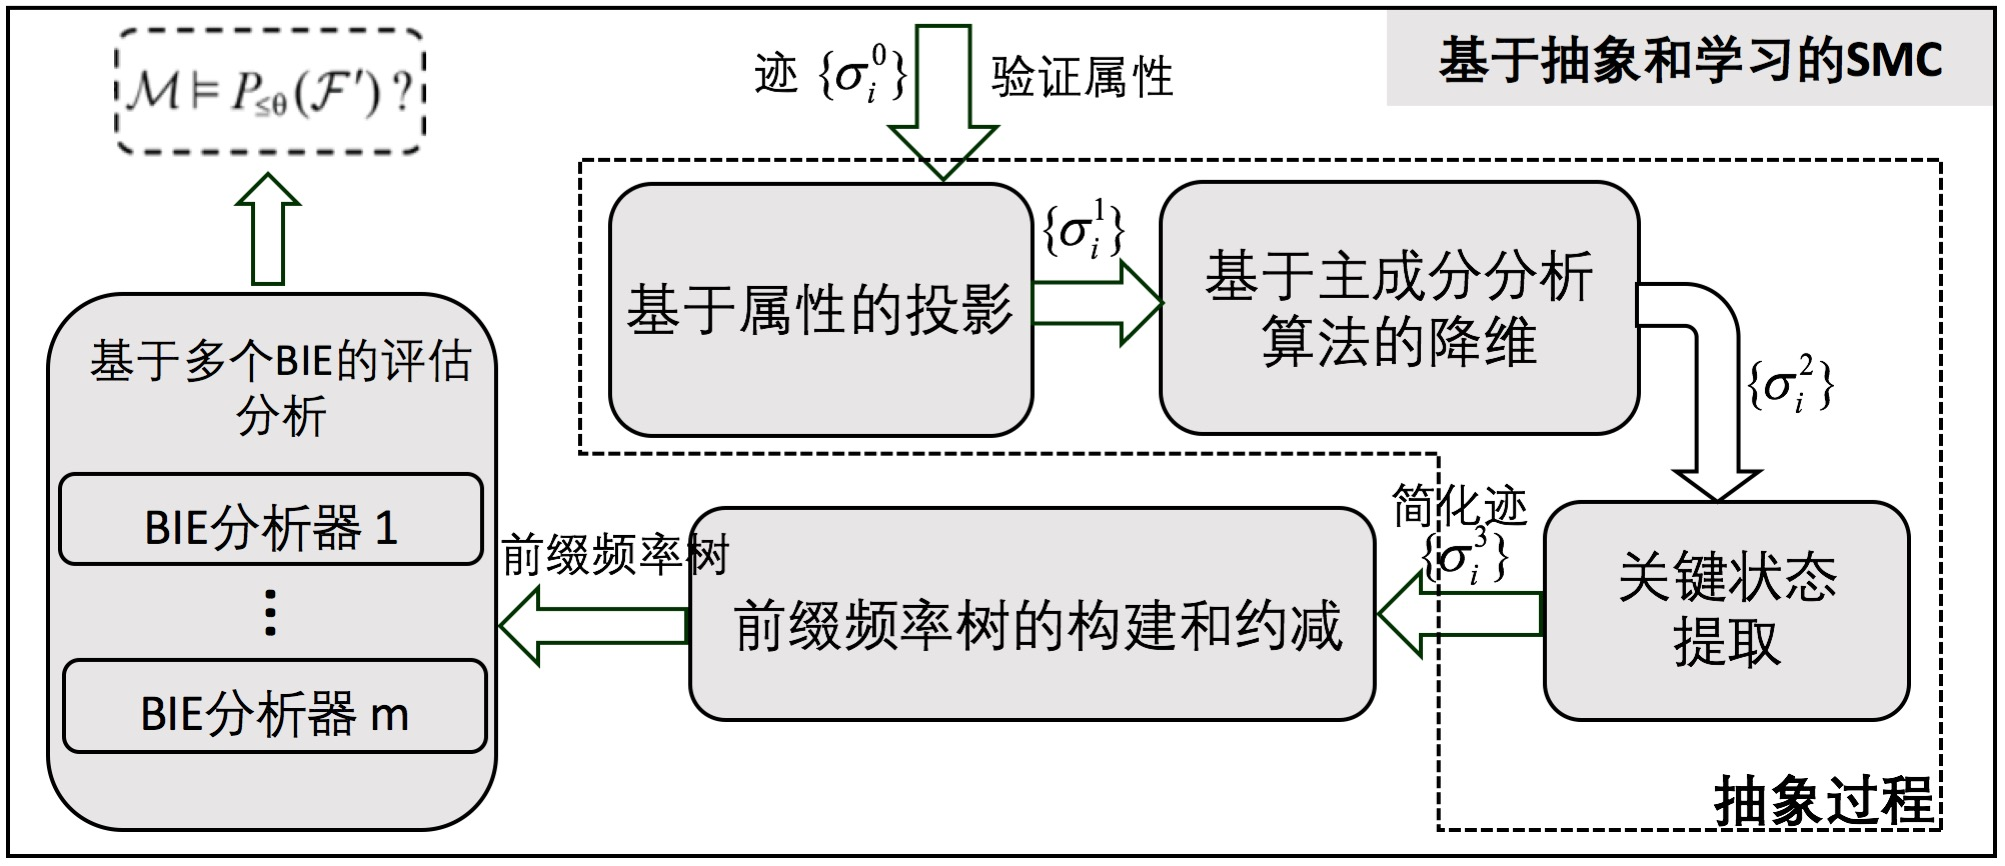
\includegraphics[width=5.0in,height=2.2in]{fig/4/ALSMC.jpg}}
	%\vspace{0.10in}
	\caption{基于抽象和学习的统计模型检测算法框架图}\label{al-smc}
\end{figure}
\subsection{基于抽象和学习的分布式统计模型检测算法}
相对于贝叶斯区间估计算法,基于抽象和学习的统计模型检测算法有效减少了验证过程中产生的仿真迹,在验证概率接近0.5时效果尤为显著。此外,我们发现该方法也可以应用本文提出的分布式框架来减少产生单条迹消耗的时间,因此我们将该方法进行了分布式设计,即得到了基于抽象和学习的分布式统计模型检测算法。该算法的主算法和从算法如算法\ref{alg:dalm}和算法\ref{alg:dals}所示。
\begin{algorithm}[t]
%\SetAlgoNoLine
\begin{algorithmic}[1]
\REQUIRE 验证属性$\phi$、模型$M$、从属节点数量$N$、抽象过程中产生的样本迹的数量 $SN$
\STATE $\sigma[0...SN-1]$ = getSampleTraces($M$)
\STATE $\sigma'[0...SN-1]$ = abstractTraces($\sigma[0...SN-1]$)
\STATE $T$ = ConstructPFT($\sigma'[0...SN-1]$)
\STATE $d$ = getSubSpacesNum($T$)
\LOOP
\STATE getConnection(slave[i])
\STATE sendModelandPropertyandPFT($M$,$\phi$,$T$,slave[i])
\IF{i>N-2}
\RETURN
\ENDIF
\ENDLOOP
\STATE x[0...d-1], n
\STATE batch[0...N-1][0...K-1][0...d-1], buffer[0...K-1], slave[0...N-1]
\end{algorithmic}
\caption{基于抽象和学习的分布式统计模型检测算法的主算法预处理}
\label{alg:dalmy}
\end{algorithm}
算法\ref{alg:dalm}是基于抽象和学习的分布式统计模型检测算法的主算法,其中$SN$是抽象过程中用到的样本迹的数量。主算法包含三个主要的步骤:(1)主算法调用仿真器产生多条样本迹$\sigma[0...SN-1]$,并将其输入到抽象过程中来得到经过抽象简化的迹$\sigma'[0...SN-1]$。然后,用简化的迹$\sigma'[0...SN-1]$构建出前缀频率树并进行约减。 (2)从属节点与主节点建立连接,主节点将模型、验证属性及前缀频率树发送给从属节点。 (3)主算法随机选择一个从算法,如果该从属节点对应的缓冲区的值小于$K$,则调用该从算法产生检测结果(相对于分布式贝叶斯区间估计算法,此时返回的是一个数组,存储着各个子模型对应的满足验证属性的批处理区的数量,而不再只是一个数值)并进行赋值。 (4)如果所有的缓冲器都不为空,则调用算法\ref{alg:sta}来计算各个子模型的估计概率$p'[j]$和后置概率$\gamma[j]$,如果某个子模型的后置概率满足$\gamma[j] > c$,则对于该子模型的验证结束。 (5)直到所有子模型的验证都结束,得到最终概率$p' := \sum\limits_{i=0}^{S-1} p[i]$,否则继续循环步骤(3)、(4)和(5)。
\begin{algorithm}[t]
%\SetAlgoNoLine
\begin{algorithmic}[1]
\REQUIRE 验证属性$\phi$、模型$M$、半区间大小$\delta \in (0, 1/2)$、区间覆盖系数$c \in (1/2, 1)$、前置beta分布的参数$\alpha$和$\beta$、缓冲区大小$K$、批处理区大小$B$、从属节点数量$N$、抽象过程中产生的样本迹的数量$SN$
\ENSURE 前缀频率树$T$、估计概率$p'$
\STATE \textbf{CallAlgorithm\ref{alg:dalmy}}
\LOOP
        \STATE node = random(0,$N$-1)
        \IF{$buffer[node] < K$}
           \STATE batch[node][buffer[node]][0...d-1] = \textbf{CallAlgorithm\ref{alg:dals}(node)}
           \STATE buffer[node]++
        \ENDIF
        \IF{$forall(i < N) buffer[i] > 0$}
        \LOOP
         \STATE x[0...d-1] += batch[i][0][0...d-1]
          \STATE n += B
           \STATE buffer[i]--
           \STATE batch[i][buffer[i]] = $\Phi$
         \IF{$i > N-1$}
         \RETURN
         \ENDIF    
         \ENDLOOP
         \ENDIF
          \STATE ter[0...d-1] = false
         \STATE  j = findUnTerminateBIE(ter[0...d-1])
          \STATE $p'[j]$,$\gamma[j]$ = \textbf{CallAlgorithm\ref{alg:sta}($\delta$, $\alpha$,$\beta$ $x[j]$, $n$)}
        \IF{$\gamma[j] > c$}
            \STATE $ter[j] = true$
         \ENDIF
         \IF{forall(ter[i] $\in$ ter[0...d-1])==true}
         \RETURN
         \ENDIF
\ENDLOOP
\RETURN $p' = \sum\limits_{i=0}^{d-1} p'[i]$
\end{algorithmic}
\caption{基于抽象和学习的分布式统计模型检测算法的主算法}
\label{alg:dalm}
\end{algorithm}
\begin{algorithm}[t]
%\SetAlgoNoLine
\begin{algorithmic}[1]
\REQUIRE 验证属性$\phi$、模型$M$、批处理区大小$B$、前缀频率树$T$、子模型数量$d$
\ENSURE 各个子模型对应的满足验证属性的迹的数量$sats[0...d-1]$
\STATE $sats[0...d-1]$, $runs$ = 0
\LOOP
        \STATE $\sigma$ = getSimulationTrace($M$)
        \STATE $\sigma'$ = abstractTrace($\sigma$)
        \IF{$\sigma \models \phi$}
           \STATE i = findSubSpace($\sigma'$, $T$)
           \STATE $sats[i]$ ++
         \ENDIF
        \STATE $runs$ ++ 
\IF{$runs$ == B}
\RETURN $sats$
\ENDIF
\ENDLOOP
\end{algorithmic}
\caption{基于抽象和学习的分布式统计模型检测算法的从算法}
\label{alg:dals}
\end{algorithm}
算法\ref{alg:dals}是基于抽象和学习的分布式统计模型检测算法的从算法。 $T$是主算法中构建并约减之后的前缀频率树。 $d$是前缀频率树叶子节点的数量,也就是划分得到的子模型的数量,$sats[i]$是第i个子模型满足验证属性的迹的数量。 从算法不断的调用仿真器产生迹$\sigma$,并将其输入到抽象过程中产生简化迹$\sigma'$。如果该迹满足验证属性,则根据前缀频率树将该迹划分给某个子模型,并更新$sats$数组。直到满足条件$runs == B$,算法终止并返回数组$sats[0...S-1]$,否则继续调用仿真器并循环。

相对于小节\ref{sec:dbie}中提出的分布式的贝叶斯区间估计算法,本算法得益于使用抽象和学习技术减少仿真迹的数量而更加高效。 然而,该算法由于使用了多个贝叶斯区间统计分析器而导致统计分析过程的误差会增大,在下面的小节,我们首先会参数优化的方法来减少该算法误差,之后给出该算法的时空复杂度及误差分析。

\subsection{参数优化}
\label{sec:opt}
在本小节我们用两种参数优化的方法来减少统计分析的误差:(1)我们发现模型划分出的子模型大小越均匀,统计分析的误差越小,因此我们用\textbf{$r$优化}来将模型划分的更加均匀。(2)用\textbf{$\delta$预测}来预测各个子模型应该用到的贝叶斯区间估计算法的半区间大小。

\textbf{$r$优化}:在基于抽象和学习的统计模型检测当中,我们通过前缀频率树的构建和约减将模型划分为了多个子模型,其中前缀频率树的叶子节点的数量即为划分得到的子模型的数量。$r$为前缀频率树的约减参数,即不同的$r$值会得到不同约减程度的前缀频率树,模型也就可能会被划分为不同数量的子模型。然而,$r$值的确定较为困难,一方面,如果$r$的值太大,我们将会得到大量的子模型导致统计分析的误差变大;另一方面,如果$r$的值太小,我们将会得到少量的子模型导致算法的效率变低。为了更好的确定$r$的值,我们采用了遗传算法\cite{DBLP:books/daglib/0019871}来获取最优的$r$值。 
\begin{equation}
\centering
\label{formula1}
r_k = M - \sum\limits_{i=1}^k \sum\limits_{j=1}^k |T_i - T_j| 
\end{equation}

假设$k$为遗传算法的种群数量,也就是在每一代划分的子模型的数量;$T_i$是第i个子模型满足验证属性的迹的数量。为了得到最优的$r$值,我们需要将模型划分的尽量均匀并要保证划分出的子模型的数量适中。因此,我们采用公式\ref{formula1} 和公式$k \geq 6 \&\& k \leq 10$分别作为遗传算法的评估函数和约束函数 。$M$是一个较大的数值,我们划分越均匀,则$\sum\limits_{i=1}^k \sum\limits_{j=1}^k |T_i - T_j|$的值越小。根据以上方法,我们可以得到最优的$r$值。

\textbf{$\delta$预测}:
经过前缀频率树的构建和约减,我们得到了多个子模型,接下来我们就可以在多个子模型上使用贝叶斯区间估计算法,每个贝叶斯区间估计算法都有自己的半区间大小$\delta$和区间覆盖系数$c$。在算法\ref{alg:dals}中,我们假设所有的贝叶斯区间估计算法都有相同的$\delta$和$c$值。然而,各个子模型最终得到的估计概率可能会有比较大的差异。例如: 我们假设所有子模型上应用的贝叶斯区间估计算法的$\delta$值都是0.1,但是可能有的子模型最终验证得到的估计概率比较小,可能还不到0.1,此时对于该子模型来说,它应用的贝叶斯区间估计算法的$\delta$值显然就不合理,并且最终会导致一个比较大的统计误差。为了解决这一问题,我们用公式\ref{formula2}所示来预测$\delta$的值。其中,$k$是子模型的数量,$T_m$是第m个子模型满足验证属性的迹的数量,$N_i$是第m个子模型上产生的总的仿真迹的数量。 $\eta$是半区间比率,本质上只是一个可以定义的参数,$\eta$越大,得到的最终估计概率约准确。应用公式\ref{formula2}来预测$\delta$之后,是得各个子模型应用贝叶斯区间估计算法得到的估计概率变得更加准确。
\begin{equation}
\label{formula2}
\delta_m = T_m / \sum\limits_{i=1}^k N_i / \eta
\end{equation}
\section{算法分析}
\subsection{时空复杂度分析}
基于抽象和学习的分布式统计模型检测算法的时空复杂度如表\ref{tb:complexity}所示。
\begin{itemize}
\item
抽象过程的时空复杂度分别为$O(mn)+O(min(k^3,n^3))$和$O(k^2)$,其中 $m$表示迹的长度,$n$表示样本迹的数量,$k$表示迹的维数。 
\item
前缀频率树构建和约减过程的时空复杂度分别为$O(mn)$ + $O(d\log{d}))$和$O(\log{d})$,其中$d$表示前缀频率树叶子节点的数量。
\item
假设贝叶斯区间估计算法迭代次数为$B$,一次统计分析的时间复杂度为$O(i)$,划分子模型需要的时间复杂度为$\log{d}$。则统计分析的时间复杂度为$O(B*(\log{d}+i))$。
\end{itemize}

\begin{table}[t]
	\caption{时空复杂度}
	\label{tb:complexity}
	\centering
	\begin{tabular}{c c c}
	    \hline
		算法过程 & 时间  & 空间 \\
		\hline
		迹的抽象 & $O(mn)$+$O(min(k^3,n^3))$ & $O(k^2)$ \\ 
		\hline
		前缀频率树 &$O(mn)$+$O(d\log{d}))$ & $O(\log{d})$ \\
		\hline
		统计分析 & $O(B*(\log{d}+i))$ & $O(1)$\\	
		\hline
	\end{tabular}
\end{table}

\subsection{误差分析}
对于特定的验证属性,模型在算法\ref{alg:dalm}的步骤(1)和(2)阶段在验证概率上是等价的。 因此,误差只出现在统计分析阶段,由于我们使用了多个贝叶斯区间估计来进行统计分析, 假设每个贝叶斯区间估计算法的半区间大小是$\delta$且子模型的数量为$M$,则此时算法的误差将不会超过$\delta*M$。此外,在小节\ref{sec:opt}中,我们还使用$\delta$预测的方法进行了算法优化,因此最终经过优化的算法误差($\xi$)满足公式\ref{formula3}。
\begin{equation}
\label{formula3}
| \xi | \leq \sum\limits_{m=1}^M (T_m / \sum\limits_{i=1}^k N_i / \eta)
\end{equation}
\section{本章小结}
本章节将上一章节经过协同仿真得到的仿真迹作为输入,使用统计模型检测算法对仿真迹进行评估分析,但是由于验证过程需要消耗大量的仿真迹且协同仿真产生一条迹本身就十分耗时。因此,我们提出了一种基于抽象和学习的分布式统计模型检测算法来提高统计模型检测的效率,并采用参数优化的方法针对该算法的误差问题进行了优化。我们已经将协同仿真引擎及改进的模型检测算法在工具中进行了实现,在下一个章节我们会给出我们工具的介绍,而对于本章提出的改进算法的效率及误差评估将会在本文的实验部分给出对比分析。